\documentclass{article}

\usepackage[usenames,dvipsnames]{color}
\usepackage{amsmath}
\usepackage{amssymb}
\usepackage{mdwlist}
\usepackage{theorem}
\newcommand{\BlackBox}{\rule{1.5ex}{1.5ex}}  
\newtheorem{example}{Example} 
\newtheorem{theorem}{Theorem}
\newtheorem{lemma}[theorem]{Lemma} 
\newtheorem{assumption}[theorem]{Assumption} 
\newtheorem{proposition}[theorem]{Proposition} 
\newtheorem{remark}[theorem]{Remark}
\newtheorem{corollary}[theorem]{Corollary}
\newtheorem{definition}[theorem]{Definition}
\newtheorem{conjecture}[theorem]{Conjecture}
\newtheorem{axiom}[theorem]{Axiom}
\usepackage[all]{xy}
\CompileMatrices
\newcommand{\eq}[1]{(\ref{#1})}
\newcommand{\mymatrix}[2]{\left[\begin{array}{#1} #2 \end{array}\right]}

%brackets
\newcommand{\inner}[2]{\left\langle #1,#2 \right\rangle}
\newcommand{\rbr}[1]{\left(#1\right)}
\newcommand{\sbr}[1]{\left[#1\right]}
\newcommand{\cbr}[1]{\left\{#1\right\}}
\newcommand{\nbr}[1]{\left\|#1\right\|}
\newcommand{\abr}[1]{\left|#1\right|}

%sets
\newcommand{\RR}{\mathbb{R}}
\newcommand{\NN}{\mathbb{N}}
\newcommand{\ZZ}{\mathbb{Z}}

%matrix stuff
\newcommand{\one}{\mathbf{1}}

%domains
\newcommand{\Bcal}{\mathcal{B}}
\newcommand{\Mcal}{\mathcal{M}}
\newcommand{\Dcal}{\mathcal{D}}
\newcommand{\Qcal}{\mathcal{Q}}
\newcommand{\Tcal}{\mathcal{T}}
\newcommand{\Fcal}{\mathcal{F}}
\newcommand{\Pcal}{\mathcal{P}}
\newcommand{\Ccal}{\mathcal{C}}
\newcommand{\Ocal}{\mathcal{O}}
\newcommand{\Xcal}{\mathcal{X}}
\newcommand{\Ical}{\mathcal{I}}
\newcommand{\Jcal}{\mathcal{J}}
\newcommand{\Ycal}{\mathcal{Y}}
\newcommand{\Gcal}{\mathcal{G}}
\newcommand{\Zcal}{\mathcal{Z}}
\newcommand{\Ncal}{\mathcal{N}}
\newcommand{\Ucal}{\mathcal{U}}
\newcommand{\Ecal}{\mathcal{E}}
\newcommand{\Hcal}{\mathcal{H}}
\newcommand{\tildi}{\tilde{\imath}}
\newcommand{\tildj}{\tilde{\jmath}}
\newcommand{\bari}{\bar{\imath}}
\newcommand{\barj}{\bar{\jmath}}

%boldface
\newcommand{\Eb}{\mathbf{E}}

%more operators
\DeclareMathOperator*{\argmax}{\mathrm{argmax}}
\DeclareMathOperator*{\argmin}{\mathrm{argmin}}
\DeclareMathOperator*{\sgn}{\mathrm{sgn}}
\DeclareMathOperator*{\tr}{\mathrm{tr}}
\DeclareMathOperator*{\cov}{\mathrm{Cov}}
\DeclareMathOperator*{\var}{\mathrm{Var}}
\DeclareMathOperator*{\mini}{\mathrm{minimize}}
\DeclareMathOperator*{\maxi}{\mathrm{maximize}}
\DeclareMathOperator*{\E}{\mathbb{E}}
\newcommand{\intset}[1]{\cbr{1..n}}
\newcommand{\flexset}[2]{\cbr{{#1}_1, \ldots, {#1}_{#2}}}

\usepackage{bm}
\usepackage{amsmath}
\usepackage{graphicx}
\usepackage[colorlinks=true,urlcolor=blue]{hyperref}
\usepackage{geometry}
\geometry{margin=1in}
\usepackage{float}
\setlength{\marginparwidth}{2.15cm}
\usepackage{booktabs}
\usepackage{enumitem}
\usepackage{epsfig}
\usepackage{setspace}
\usepackage{parskip}
\usepackage[]{algorithm2e}
\usepackage{comment}
\usepackage{pdfpages}
\usepackage{physics}
\usepackage{color}
\usepackage{ulem}
\usepackage{bbm}

%\newcommand{\comment}[1]{\textcolor{blue}{\textsc{\textbf{[#1]}}}}
\def\R{\mathbb{R}}
\def\T{^\intercal}
\newcommand{\st}{\mathop{\mathrm{subject\,\,to}}}

\makeatletter
\newcommand{\removelatexerror}{\let\@latex@error\@gobble}
\makeatother

\begin{document}

\section*{}
\begin{center}
  \centerline{\textsc{\LARGE Homework 2}}
  \vspace{0.5em}
  \centerline{\textsc{\Large Na{\"i}ve Bayes; SVM}}
  \vspace{1em}
  \textsc{\large CMU 10-701: Machine Learning (Spring 2017)} \\
  \vspace{1em}
  \centerline{OUT: Feb 13}
  \centerline{DUE: \sout{Feb 23} \textcolor{red}{Feb 27}, 11:59 PM}
\end{center}
\graphicspath{images}

\section*{START HERE: Instructions}


\begin{itemize*}

\item \textbf{Collaboration policy:} Collaboration on solving the homework is allowed, after you have thought about the problems on your own.  It is also OK to get clarification (but not solutions) from books or online resources, again after you have thought about the problems on your own.  There are two requirements: first, cite your collaborators fully and completely (e.g., ``Jane explained to me what is asked in Question 3.4'').  Second, write your solution {\em independently}: close the book and all of your notes, and send collaborators out of the room, so that the solution comes from you only.



\item\textbf{Submitting your work:} Assignments should be submitted as PDFs using Gradescope unless explicitly stated otherwise.  Each derivation/proof should be completed on a separate page. Submissions can be handwritten, but should be labeled and clearly legible.  Else, submissions can be written in LaTeX.  Upon submission, label each question using the template provided by Gradescope.

 \item \textbf{Programming}: All programming portions of the assignments should be submitted to Gradescope as well.  We will not be using this for autograding, but rather for plagiarism detection, meaning you may use any language which you like to submit.
\end{itemize*}

\newpage


\section*{Part A : Multiple Choice Questions[8 points] (Yichong)}

\begin{itemize}
	\item \textbf{There might be one or more right answers}. Please explain your choice in one or two sentences.
\end{itemize}

\vspace {2mm}

\begin{enumerate}

		\item \textbf{[This is to remind you that there might be one or more answers.]} Which of the following is(are) \emph{not} one of the TAs of this class?\\
		A. Yichonnnnnnnng Xu\\
		B. Ademacia Yu\\
		C. Danish Schwartz\\
		D. Pradeep Prakhar Naval\\		
		\textbf{Answer: \underline{B}}

		\item \textbf{[2 Points]} Which of the following methods is(are) model-based method(s)? \\ \\
		A. Support Vector Machines \\
		B. Logistic Regression\\
		C. Naive Bayes\\
		D. Linear Regression\\
		\textbf{Answer: \underline{C}}\\
		SVM, logistic regression, and linear regression do not have assumptions on probabilistic models of their likelihood or prior distribution. The Naive Bayes has assumptions on both class conditional likelihood and class prior distribution.

		\item \textbf{[2 Points]} Suppose we are learning a Naive Bayes model on a 2-dimensional binary data using MLE estimation. That is, we are learning a naive Bayes classifier from $X\in \{0,1\}^2$ to $Y\in \{0,1\}$. Suppose the training data is $((0,0),1), ((0,1),1),((1,1),1),((1,1),0),((0,0),0)$. What is the maximum likelihood estimation(MLE) probability of $P(Y=1|X=(1,0))$ under the Naive Bayes model?\\
		A. $\frac{2}{5}$. \ \ \ \ \  B. $\frac{1}{3}$. \ \ \ \ \  C. $\frac{3}{5}$. \ \ \ \ \ D. $\frac{11}{18}$.
		\\
		\textbf{Answer: \underline{A}}
		
		\begin{equation}
		\nonumber
		\begin{array}{rcl}
		P(Y=1|X=(1,0)) & = & \frac{P(X=(1,0)|Y=1)P(Y=1)}{P(X=(1,0))} \\
					   & = & \frac{P(X_0=1|Y=1)P(X_1=0|Y=0)P(Y=1)}{P(X_0=1|Y=1)P(X_1=0|Y=0)P(Y=1)+P(X_0=1|Y=0)P(X_1=0|Y=0)P(Y=0)} \\
					   & = & \frac{1/3\times1/3\times3/5}{1/3\times1/3\times3/5+1/2\times1/2\times2/5} \\
					   & = & \frac{2}{5}
		\end{array}
		\end{equation}

		\item \textbf{[2 Points]} For each of the following loss functions, which one is(are) non-convex in $f(x)$? \\ \\
		A. 0-1 loss: $l(y,f(x))=1_{y\ne f(x)}$. \\
		B. Mean squared error: $l(y,f(x))=(y-f(x))^2$.  \\
		C. The hinge loss: $l(y,f(x))=\max(0,1-yf(x))$. \\
		D. The logistic loss: $l(y,f(x))=\log(1+\exp(-yf(x)))$. \\
		\\
		\textbf{Answer: \underline{A}}\\
		A is equivalent to a $\delta$ function $\delta(f(x)-y)$; therefore, it is a non-convex function.
		
		\item \textbf{[2 points]} Suppose we use the following form of SVM on a dataset $\{(x_i,y_i)\}_{i=1}^n$:
		\begin{align*}
		\text{minimize}\; & \frac{1}{n}\sum_{i=1}^n \xi_i+\lambda\|w\|_2^2\\
		\text{subject to } & y_i(w^Tx_i+b)\geq 1-\xi_i, \xi_i\geq 0, i=1,2,...,n.
		\end{align*}
		Suppose we have $\xi_1=1, \xi_2=0, \xi_3=2$ at the optimal solution. Which of the following statements is(are) true for the optimal classifier?\\
		A. $x_1$ lies on the decision boundary.\\
		B. $x_2$ lies on the decision boundary.\\
		C. $x_2$ lies on the wrong side of the decision boundary (i.e., $y_2$ is of a different sign as the classifier prediction.).\\
		D. $x_3$ lies on the wrong side of the decision boundary (i.e., $y_3$ is of a different sign as the classifier prediction.).\\
		\textbf{Answer: \underline{A,D}}\\
		\begin{itemize}
			\item $\xi=0$: the data point $\vec{x}_i$ and its label $y_i$ satisfy $y_i(\vec{w}^T\vec{x}_i+b) \geq 1$, which means $\vec{x}_i$ is correctly classified.
			\item $0<\xi\leq1$: the data point $\vec{x}_i$ and its label $y_i$ satisfy $0\leq y_i(\vec{w}^T\vec{x}_i+b) <1$, which means $\vec{x}_i$ is correctly classified but within margin area.
			\item $1<\xi$: the data point $\vec{x}_i$ and its label $y_i$ satisfy $y_i(\vec{w}^T\vec{x}_i+b) <0$, which means $\vec{x}_i$ is not correctly classified (on the wrong side of the decision boundary).
		\end{itemize}

	\end{enumerate}
	\clearpage


\section*{Part B, Problem 1: Na{\"i}ve Bayes[20 Points] (Adams and Danish)}

In this question, we use upper-case letters such as $X,Y$ to denote random variables, and lower-case letters to denote values of random variables.

Suppose we want to model the probability distribution $P(Y|X)$ (or equivalently $P(X,Y)$), with $X=(X_1,X_2,..,.X_n)$, where $Y\in \{0, 1\}$ is the label, and $X_i, i=1,2,...,n$ are the features. Remember that
\begin{equation}\label{eqn:pxy}
P(Y|X)\propto P(X|Y)P(Y),
\end{equation}
so we are essentially modeling $P(X|Y)$ and $P(Y)$.
%\begin{equation}
%P(X|Y)P(Y).
%\end{equation}


\begin{enumerate}
\item\textbf{[1 points]}  \sout{Given} \textcolor{red}{Give} the Na{\"i}ve Bayes formulation of \eqref{eqn:pxy} under the assumption that features are conditional independent given the label.\\
\textbf{Answer:}\\
\begin{equation}
\nonumber
\begin{array}{rcl}
P(Y|X) & \propto & P(X|Y)P(Y) \\
	   & = & P(X_1,X_2,\dots,X_n|Y)P(Y) \\
	   & = & P(X_1|X_2,\dots,X_n,Y)P(X_2,\dots,X_n|Y)P(Y) \\
	   & = & P(X_1|Y)P(X_2,\dots,X_n|Y)P(Y) \\
	   & \dots & \\
	   & = & \prod_{i=1}^{n} P(X_i|Y) P(Y)
\end{array}
\end{equation}



\item\textbf{[4 points]} Suppose each feature $X_i$ takes values from $\{1,2,...,K\}$. Let's assume the label distribution is Bernoulli and the feature distribution conditioned on label is multinomial. What is the total number of parameters of the model with Na{\"i}ve Bayes assumption? What about the model without the assumption? Please give detailed derivation step by step.\\
\textbf{Answer:}\\
\begin{itemize}
	\item With Na{\"i}ve Bayes assuption:\\
	For the class prior distribution $P(Y)$ following Bernoulli distribution, it contains 1 parameter. For the class conditional distribution $P(X|Y)=\prod_{i=1}^{n} P(X_i|Y)$ following multinomial distribution, each $P(X_i|Y)$ contains $K-1$ parameters; therefore the total number of parameters for $P(X|Y)$ is $2n(K-1)$ (2 classes). So the total number of parameters of the model with Na{\"i}ve Bayes assumption is $\underline{2n(K-1)+1}$
	\item Without Na{\"i}ve Bayes assuption:\\
	For class prior distribution $P(Y)$, it still contains 1 parameter. For the class conditional distribution $P(X|Y)$ following multinomial distribution, the total number of possible value of $X$ is $K^n$, and thus $P(X|Y)$ needs $2(K^n-1)$ parameters (2 classes). So the totoal number of parameters of the model without Na{\"i}ve Bayes assumption is $\underline{2(K^n-1)+1}$
	
\end{itemize}


\item\textbf{[6 points]} Suppose each feature $X_i$ takes values from $\{0,1\}$. Let's assume the label distribution is Bernoulli and the feature distribution conditioned on label is \sout{multinomial} \textcolor{red}{Bernoulli}. Let $\pi = P(Y=1)$ and $\mu_{ijk}=P(X_i=k|Y=j)$, for $i=1,2,...,n$, $k=0,1$ and $j=0,1$. Given $N$ observations $\{(X^{p},Y^{p})\}_{p=1}^N$, derive the MLE estimators of $\pi$ and $\mu_{ijk}$.\\
\textbf{Answer:}\\
\begin{equation}
\nonumber
\begin{array}{rcl}
\pi & = & \frac{\sum_{p=1}^{N} 1_{(Y^p=1)}}{N} \\
\mu_{ijk} & = & \frac{\sum_{p=1}^{N}1_{(X_i^p=k)}1_{(Y^p=j)}}{\sum_{p=1}^{N}1_{(Y^p=j)}} \\
\end{array}
\end{equation}

\item Suppose each feature $X_i\in\mathbb{R}$ and  $P(X_i|Y=j)\sim \mathcal{N}(\theta_{ij}, 1)$ for $i=1,2,...,n$ and $j=0,1$.

\begin{enumerate}
\item\textbf{[3 points]} Given $N$ observations $\{(X^{p},Y^{p})\}_{p=1}^N$, derive the MLE estimator of $\theta_{ij}$.\\
\textbf{Answer:}\\

\begin{equation}
\begin{array}{rcl}
\theta_{ij} & = & \frac{\sum_{p=1}^{N}1_{(Y^p=j)}X_i^p}{\sum_{p=1}^{N}1_{(Y^p=j)}}
\end{array}
\end{equation}

\item\textbf{[6 points]} Show that the decision boundary $\{X_1,X_2,...,X_n: P(Y=0|X_1,X_2,...,X_n) = P(Y=1|X_1,X_2,...,X_n)\}$ is linear in $X_1,X_2,...,X_n$.\\
\textbf{Answer:}\\

$\because$ $P(X_i|Y=j)=\frac{1}{\sqrt{2\pi}}\exp(-\frac{(X_i-\theta_{ij})^2}{2})$\\
$\therefore$ $\forall$ $X=\{X_1,X_2,\dots,X_n\}$ on the decision boundary, then:
\begin{equation}
\nonumber
\begin{array}{rcl}
P(Y=0|X) & = & P(Y=1|X) \\
\frac{\prod_{i=1}^{n}P(X_i|Y=0)}{\prod_{i=1}^{n}P(X_i|Y=1)} & = & \frac{P(Y=1)}{P(Y=0)} \\
\frac{1}{2}\sum_{i=1}^{n}((X_i-\theta_{i0})^2-(X_i-\theta_{i1})^2) & = & \ln(\frac{\pi}{1-\pi}) \\
\sum_{i=1}^{n}(\theta_{i1}-\theta_{i0})(2X_i-\theta_{i0}-\theta_{i1}) & = & 2\ln(\frac{\pi}{1-\pi}) \\
\sum_{i=1}^{n}(\theta_{i1}-\theta_{i0})X_i + \frac{1}{2}\sum_{i=1}^{n}(\theta_{i0}^2-\theta_{i1}^2)-\ln(\frac{\pi}{1-\pi}) & = & 0 \\
\end{array}
\end{equation}
$\therefore$ The decision boundary is linear in $X_1,X_2,...,X_n$.

\end{enumerate}

\end{enumerate}


\newpage


\section*{Part B, Problem 2: Support Vector Machine (25 pts) (Hao and Prakhar)}
Suppose we have the following data $$\mathcal{D} = (\mathbf{X},\mathbf{y})$$ where $\mathbf{X} \in \mathbb{R}^{d \times n}$, the $i$-th column $x_i$ are the features of the $i$-th training sample and $y_i$ is the label of the $i$-th training sample.
$\mathbf{y} \in \left\{-1,1\right\}^n$ if this is a classification problem and $\mathbf{y} \in \mathbb{R}^n$ if this is a regression problem.


\subsection*{2.1 SVM for Classification (15 pts)}
\begin{enumerate}

\item\textbf{[5 points]} (1) In the linearly separable case if one of the training samples is removed, will the decision boundary shift toward the point removed or shift away from the point removed or remain the same? (2) Now if we consider that the decision boundary is of Logistic Regression, will the decision boundary change or remain the same? Explain you answer. (No need to mention the direction of change in (2)) \\
\textbf{Answer:}\\
\begin{itemize}
	\item In the linearly separable case ($\vec{w}=\sum_i^n{\alpha_i y_i \vec{X}^{(i)}}$, $b=\sum_{i=1}^n{\alpha_i y_i}$, $\sum_{i=1}^n\alpha_i=1$, $\alpha_i\geq0$), all data points are on the correct side of the decision boundary and not within margin area; therefore if the removed point is on the margin ($\alpha_i>0$), the decision boundary may shift toward the removed point after retraining, but if the removed point is not on the margin ($\alpha_i=0$), the decision boundary will remain the same.
	\item For logistic regression, the decision boundary is decided by all data points; therefore, removing a point will eventually change the decision boundary.
\end{itemize}

%\begin{soln}
%Solution: \\

%\end{soln}


\item Recall from the lecture notes that if we allow some misclassification in the training data, the primal optimization of SVM (soft margin) is given by
$$
\begin{aligned}
& \underset{w, \xi_i}{\text{minimize}} && \frac{1}{2}||w||_2^2 + C\sum_{i=1}^n\xi_i\\
& \text{subject to} && y_i(w^Tx_i) \geq 1-\xi_i & \forall i = 1,\ldots, n\\
& && \xi_i \geq 0 & \forall i = 1,\ldots, n
\end{aligned}
$$

where $\xi_1,\ldots, \xi_n$ are called slack variables.
% The optimal slack variables have intuitive geometric interpretation as shown below:
%
% \begin{figure}[H]
% 	       \centering
% 	       \includegraphics[width=0.4\textwidth]{Untitled.png}
% 	       \caption{}
% 	       \label{fig:my_label}
% \end{figure}

	(1) \textbf{[3 points]} Suppose the optimal $\xi_1,\ldots,\xi_n$ have been computed. Use the $\xi_i$ to obtain an upper bound on the number of misclassified instances.\\
	\textbf{Answer:}\\
	$$\sum_{i=1}^n 1_{(\xi_i>1)}$$

%	\begin{soln}
%		Solution: \\

%	\end{soln}


	(2) \textbf{[3 points]} In the primal optimization of SVM, what's the role of the coefficient $C$?
	Briefly explain your answer by considering two extreme cases, i.e., $C\rightarrow 0$ and $C\rightarrow\infty$.\\
	\textbf{Answer:}\\
	The $C$ controls the tolerance of error in the SVM model. If $C \rightarrow 0$, the SVM model will ignore any misclassification error. If $C \rightarrow \infty$, the SVM model will not tolerate any misclassification error.

%	\begin{soln}
%		Solution: \\

%	\end{soln}

	\item\textbf{[2 points]} Compare Hard SVM and Logistic Regression when the two classes are linearly separable. Give any significant differences. (*Hint* - think in terms of decision boundary)\\
	\textbf{Answer:}\\
	Hard SVM tries to find the separating hyperplane to maximize the distance of the closest points to the margin. Logistic regression focuses on maximizing the probability of the data. If the data from different classes are unbalanced, the hard SVM's boundary will not be affected for the support vectors, but the logistic regression's boundary will prefer the class with fewer data.

%	\begin{soln}
%		Solution: \\

%	\end{soln}

	\item\textbf{[2 points]} Compare Soft SVM and Logistic Regression when the two classes are not linearly separable. Give any significant differences.\\
	\textbf{Answer:}\\
	Soft SVM tries to find the separating hyperplane to maximize the distance of the closest points to the margin as well as to minimize the classification error via hinge loss function. Logistic regression only focuses on maximizing the probability of the data via logistic loss.

%	\begin{soln}
%		Solution: \\

%	\end{soln}


\end{enumerate}




\subsection*{2.2 SVM for Regression (10 pts)}
Let $x \in \mathbb{R}^d$ be the feature vector and $y \in \mathbb{R}$ be the label.
In this question, we use a linear predictor for the label, i.e. given the feature vector, we predict the label by \[
\hat{y}\left(x\right) = w^\top x
\] where $w \in\mathbb{R}^d$ is the linear coefficient vector.
In this question, we consider the \textbf{epsilon insensitive loss function}, defined by\begin{align*}
L_{\epsilon}\left(y,\hat{y}\right) = \begin{cases}
0 \qquad &\text{if } \abs{y-\hat{y}} < \epsilon \\
\abs{y-\hat{y}} - \epsilon \qquad &\text{otherwise}.
\end{cases}
\end{align*} where $\epsilon$ is a tuning parameter.
To obtain a good $w$, we would like to solve the following optimization:
\begin{align}
J\left(w\right) = \frac{1}{n}\sum_{i=1}^{n}L_\epsilon\left(y,\hat{y}\left(x_i\right)\right) + \lambda\norm{w}_2^2. \label{eqn:svr}
\end{align}
\begin{enumerate}
\item\textbf{[2 points]} \sout{What kind of loss is $L_ε$ if $ε = 0$?} \textcolor{red}{ When $\epsilon$ = 0, is the loss function the same as the absolute error loss? Show why. What role do you think $\epsilon$ plays?}  \\
\textbf{Answer:}\\
Yes. When $\epsilon$ = 0, $L_\epsilon(y,\hat{y})=|y-\hat{y}|$. The $\epsilon$ controls the region around $y$ where $\hat{y}$ should fall.

%\begin{soln}
%	Solution: \\

%\end{soln}

\item\textbf{[8 points]} Notice that~\eqref{eqn:svr} is not a differentiable objective.
Show how to convert \eqref{eqn:svr} into a optimization problem whose objective is differentiable and constraints are linear by introducing slack variables. \\

\textbf{Answer:}\\

$$\argmin_{\vec{w}} ||\vec{w}||_2^2 + C\sum_{i=1}^{n}\Delta_i$$
s.t.
$$y_i-\vec{w}^T\vec{x}_i \leq \epsilon+\Delta_i$$
$$y_i-\vec{w}^T\vec{x}_i \geq -\epsilon-\Delta_i$$
$$\Delta_i\geq0$$

%\begin{soln}
%	Solution: \\
%\end{soln}

\end{enumerate}

\newpage


\section*{Part B, Problem 3: Minimum Enclosing Ball [20 Points] (Calvin and Dan)}

Consider a set of data points $\{\boldsymbol{z}_1,\dotsc,\boldsymbol{z}_n\}$ with $\boldsymbol{z}_i \in \R^p$. In this problem, we would like to find the center $\boldsymbol{c}$ and radius $R$ of the smallest ball that contains all of the data. We can formalize this optimization problem by minimizing the square of this radius while constraining the squared distance between $\boldsymbol{z}_i$ and $c$ to be less than $R^2$ as in Equation~\ref{eq:hard_ball}
\begin{align}
\argmin_{R,\boldsymbol{c}}&\quad R^{2} \nonumber \\ \st&\quad\norm{\boldsymbol{c}-\boldsymbol{z}_{i}}_{2}^{2}\leq R^{2}\quad \forall i=1,\dotsc,n \label{eq:hard_ball} 
\end{align}
\begin{enumerate}
\item \textbf{[1 points]} Write the Lagrangian $\mathcal{L}(R, \boldsymbol{c}, \boldsymbol{\alpha})$ using $\alpha_i$ for dual variables associated with the distance constraints.\\
\textbf{Answer:}\\
\begin{equation}
\nonumber
\begin{array}{rcl}
L(R,\vec{c},\vec{\alpha}) & = & R^2 + \sum_{i=1}^n\alpha_i(||\vec{C}-\vec{z}_i||_2^2-R^2)
\end{array}
\end{equation}

\item \textbf{[2 points]} Derive and write down the dual optimization problem for this primal problem.\\
\textbf{Answer:}\\
$\because$
\begin{equation}
\nonumber
\begin{array}{rcl}
\partial \mathcal{L}(R,\vec{c},\vec{\alpha}) / \partial R & = & 2R(1 - \sum_{i=1}^n\alpha_i) = 0 \\
			& \Rightarrow & \sum_{i=1}^n\alpha_i=1 \\
\partial \mathcal{L}(R,\vec{c},\vec{\alpha}) / \partial \vec{c} & = & 2\sum_{i=1}^n\alpha_i(\vec{c}-\vec{z}_i) = 0 \\
			& \Rightarrow & \vec{c}=\sum_{i=1}^n\alpha_i\vec{z}_i \\
\end{array}
\end{equation}
$\therefore$
$$L(R^*,\vec{c}^*,\vec{\alpha}) = \sum_{i=1}^n \alpha_i||\vec{z}_i||_2^2 - ||\sum_{i=1}^n\alpha_i\vec{z}_i||_2^2$$
$$\argmin_{\vec{\alpha}} ||\sum_{i=1}^n\alpha_i\vec{z}_i||_2^2 - \sum_{i=1}^n \alpha_i||\vec{z}_i||_2^2$$
s.t.
$$\sum_{i=1}^n\alpha_i=1$$
$$\alpha_i \geq 0$$

\end{enumerate}
 
To account for noise and outliers, we introduce non-negative slack variables $\zeta_i$ and constrain the squared distance between $\boldsymbol{z}_i$ and $\boldsymbol{c}$ to be less than $R^2 + \zeta_i$ for all $i=1,\dotsc,n$. This can be formalized with the optimization problem in Equation~\ref{eq:soft_ball}, where a hyperparameter $\eta$ controls the tradeoff between the size of the ball and the number of points not enclosed within it. 
\begin{align}
\argmin_{R,\boldsymbol{c},\boldsymbol{\zeta}}&\quad R^{2}+\eta \sum_{i=1}^{n} \zeta_i \nonumber \\ \st&\quad\left\Vert \boldsymbol{c}-\boldsymbol{z}_{i}\right\Vert _{2}^{2}\leq R^{2}+\zeta_{i}\quad \forall i=1,\dotsc,n \label{eq:soft_ball} \\
&\quad \zeta_{i}\geq0\quad \forall i=1,\dotsc,n \nonumber
\end{align}

\begin{enumerate}[resume]
\item \textbf{[1 points]} Write the Lagrangian $\mathcal{L}(R, \boldsymbol{c}, \boldsymbol{\zeta}, \boldsymbol{\alpha}, \boldsymbol{\gamma})$ using $\alpha_i$ for dual variables associated with the distance constraints and $\gamma_i$ for dual variables associated with the slack variable constraints.\\
\textbf{Answer:}\\
\begin{equation}
\nonumber
\begin{array}{rcl}
L(R,\vec{c},\vec{\alpha}) & = & R^2 + \eta \sum_{i=1}^n \xi_i + \sum_{i=1}^n\alpha_i(||\vec{C}-\vec{z}_i||_2^2-R^2-\xi_i) - \sum_{i=1}^n\gamma_i\xi_i
\end{array}
\end{equation}

\item \textbf{[2 points]} Derive and write down the dual optimization problem for this primal problem. \\
\textbf{Answer:}\\
$\because$
\begin{equation}
\nonumber
\begin{array}{rcl}
\partial L(R, \boldsymbol{c}, \boldsymbol{\zeta}, \boldsymbol{\alpha}, \boldsymbol{\gamma}) / \partial R & = & 2R(1 - \sum_{i=1}^n\alpha_i) = 0 \\
				& \Rightarrow & \sum_{i=1}^n\alpha_i=1 \\
\partial L(R, \boldsymbol{c}, \boldsymbol{\zeta}, \boldsymbol{\alpha}, \boldsymbol{\gamma}) / \partial \vec{c} & = & 2R(1 - \sum_{i=1}^n\alpha_i) = 0 \\
				& \Rightarrow & \vec{c}=\sum_{i=1}^n\alpha_i\vec{z}_i \\
\partial L(R, \boldsymbol{c}, \boldsymbol{\zeta}, \boldsymbol{\alpha}, \boldsymbol{\gamma}) / \partial \vec{\xi_i} & = &  \eta - \alpha_i - \gamma_i = 0 \\
				& \Rightarrow & \eta = \alpha_i + \gamma_i \\
\end{array}
\end{equation}
$\therefore$
$$L(R^*, \boldsymbol{c}^*, \boldsymbol{\zeta}^*, \boldsymbol{\alpha}, \boldsymbol{\gamma}) = \sum_{i=1}^n \alpha_i||\vec{z}_i||_2^2 - ||\sum_{i=1}^n\alpha_i\vec{z}_i||_2^2$$
$$\argmin_{\vec{\alpha}} ||\sum_{i=1}^n\alpha_i\vec{z}_i||_2^2 - \sum_{i=1}^n \alpha_i||\vec{z}_i||_2^2$$
s.t.
$$\sum_{i=1}^n\alpha_i=1$$
$$\eta \geq \alpha_i \geq 0$$

\end{enumerate}


Let us stipulate that strong duality holds for the primal and dual problems described by Equation~\ref{eq:soft_ball}. Then if we call our primal criterion function $f$ and a solution to our primal problem ($R^{*}$, $\boldsymbol{c}^{*}$, and $\boldsymbol{\zeta}^{*}$) and we call our dual criterion function $g$ and a solution to our dual problem $\boldsymbol{\alpha}^{*}$, we have:
\begin{align*}
    f(R^{*}, \boldsymbol{c}^{*}, \boldsymbol{\zeta}^{*}) =& g(\boldsymbol{\alpha}^{*}) \\
    =& \mathop{\mathrm{min}}_{R,\boldsymbol{c}, \boldsymbol{\zeta}} \left[ f(R, \boldsymbol{c},\boldsymbol{\zeta}) + \sum_{i=1}^{n} \alpha_i^{*} h_i(R, \boldsymbol{c}, \boldsymbol{\zeta}) \right] \\
    &\le f(R^{*}, \boldsymbol{c}^{*}, \boldsymbol{\zeta}^{*}) + \sum_{i=1}^{n} \alpha_i^{*} h_i(R^{*}, \boldsymbol{c}^{*}, \boldsymbol{\zeta}^{*}) \\ 
    &\le f(R^{*}, \boldsymbol{c}^{*}, \boldsymbol{\zeta}^{*})
\end{align*}
Where $h_i(R, c, \boldsymbol{\zeta})$ is a constraint. This means that all of the inequalities above are equalities, which implies that $\sum_{i=1}^{n} \alpha_i^{*} h_i(R^{*}, \boldsymbol{c}^{*}, \boldsymbol{\zeta}^{*}) = 0$. Since we know from the definition of the Lagrangian that $h_i(R, \boldsymbol{c}, \boldsymbol{\zeta}) \ge 0$ and $\alpha_i \ge 0$, each term here is non-negative. This further implies that each individual term must be 0, i.e. we know:
\begin{align*}
    \alpha_i^{*} h_i(R^{*}, \boldsymbol{c}^{*},\boldsymbol{\zeta}^{*}) = 0\quad \forall i \in {1,\dotsc,n}
\end{align*}
This is a general principle of strong duality called complementary slackness: for a given $i$, at least one of the dual variable $\alpha_i$ and the constraint $h_i$ must evaluate to 0 at the solution.
\begin{enumerate}[resume]
\item \textbf{[2 points]} Using the principle of complementary slackness, for the form of the problem in Equation~\ref{eq:soft_ball}, describe boundary conditions on each $\alpha_i$. From the values of $\alpha_i$, when is a point $\boldsymbol{z}_i$ exactly on the boundary of the hypersphere?\\
\textbf{Answer:}\\

From the complementary slackness, we know that if $h_i(R,\vec{c},\vec{\zeta})=0$, then $\alpha_i$ can be positive, otherwise, $\alpha_i=0$. Because $\sum_{i=1}^n\alpha_i=1$, $\exists \alpha_k,$ that $\eta>\alpha_k>0$; therefore, the corresponding constraint $h_k(R,\vec{c},\vec{\zeta})=0$, which implies $\vec{z}_k$ is on the boundary. With $\vec{c}=\sum_{i=1}^n\alpha_i\vec{z}_i$, the ball's boundary can be determined uniquely.

\item \textbf{[2 points]} What is the solution to the primal problem in Equation~\ref{eq:soft_ball} in terms of the solution to the dual problem?\\
\textbf{Answer:}\\
$$\vec{c}=\sum_{i=1}^n\alpha_i\vec{z}_i$$
$$R^2=||\vec{z}_k-\vec{c}||~~~~where,~\eta>\alpha_k>0$$



\end{enumerate}

The structure of the dual problem should look very similar to that of the soft-margin support vector 
machine (SVM). In fact, we will show that a variation of the soft-margin SVM called the L2-SVM can be equivalently interpreted 
as a minimum enclosing ball problem if the input data is normalized to unit length.

Consider a set of data points $\{\left(\boldsymbol{x}_1,y_1\right),\dotsc,\left(\boldsymbol{x}_n,y_n\right)\}$ where $\boldsymbol{x}_i \in \R^p$, $\left\Vert \boldsymbol{x}_{i}\right\Vert=1$, and $y_i \in \left\{-1,1\right\}$ for all $i=1,\dotsc,n$ . In the L2-SVM formulation in Equation~\ref{eq:l2svm}, we explicitly maximize the margin $\rho$ and penalize the square of the intercept $b$ along with the squares of the slack variables $\xi_i$ so that we no longer need to constrain them to be non-negative. 
\begin{align}
    \min_{\boldsymbol{w}, \boldsymbol{\xi}, \rho}&\quad \frac{1}{2} \norm{\boldsymbol{w}}_2^2 + \frac{1}{2}b^2- \rho + \frac{\lambda}{2} \sum_{i=1}^n \xi_i^2 \nonumber\\
    \st&\quad y_i(w\T \boldsymbol{x_i} + b) \ge \rho - \xi_i,\quad i = 1,\dotsc,n \label{eq:l2svm}		
\end{align}
\begin{enumerate}[resume]
    \item \textbf{[4 points]} Derive the dual for the L2-SVM problem in Equation~\ref{eq:l2svm}.\\
    \textbf{Answer:}\\
    $\because$
    \begin{equation}
    \nonumber
    \begin{array}{rcl}
    L(\vec{w},\vec{\xi},\rho,\vec{\alpha}) & = & \frac{1}{2}||\vec{w}||_2^2 + \frac{1}{2}b^2 - \rho + \frac{\lambda}{2}\sum_{i=1}^{n}\xi_i^2-\sum_{i=1}^{n}\alpha_i(y_i(\vec{w}^T\vec{x}_i+b)-\rho+\xi_i) \\
    \partial L(\vec{w},\vec{\xi},\rho,\vec{\alpha}) / \partial \vec{w} & = & \vec{w} - \sum_{i=1}^{n}\alpha_iy_i\vec{x}_i = 0 \\
    			& \Rightarrow & \vec{w} = \sum_{i=1}^{n}\alpha_iy_i\vec{x}_i \\
    \partial L(\vec{w},\vec{\xi},\rho,\vec{\alpha}) / \partial \xi_i & = & \lambda\xi_i - \alpha_i = 0 \\
    			& \Rightarrow & \xi_i=\frac{\alpha_i}{\lambda} \\
    \partial L(\vec{w},\vec{\xi},\rho,\vec{\alpha}) / \partial \rho & = &  -1 + \sum_{i=1}^{n}\alpha_i = 0 \\
    			& \Rightarrow & \sum_{i=1}^{n}\alpha_i = 1 \\
    \end{array}
    \end{equation}
    $\therefore$
    $$L(\vec{w}^*,\vec{\xi}^*,\rho^*,\vec{\alpha}) = -\frac{1}{2}||\sum_{i=1}^{n}\alpha_iy_i\vec{x}_i||_2^2 - \frac{1}{2}(\sum_{i=1}^{n}\alpha_iy_i)^2 - \frac{1}{2\lambda}\sum_{i=1}^{n}\alpha_i^2 $$
    $$\argmin_{\vec{\alpha}}||\sum_{i=1}^{n}\alpha_iy_i\vec{x}_i||_2^2 + (\sum_{i=1}^{n}\alpha_iy_i)^2 + \frac{1}{\lambda}\sum_{i=1}^{n}\alpha_i^2 $$
    s.t.
    $$\sum_{i=1}^{n}\alpha_i=1$$
    $$\alpha_i \geq 0$$
    
	\item \textbf{[4 points]} Show that the dual of this problem is equivalent to the dual of the hard minimum enclosing ball problem in Equation~\ref{eq:hard_ball} when the data is augmented as follows:
	\[\boldsymbol{z}_{i}=\left[\begin{array}{c}
	y_{i}\boldsymbol{x}_{i}\\
	y_{i}\\
	\frac{1}{\sqrt{\lambda}}\boldsymbol{e}_{i}
	\end{array}\right]\]
	(Note that $\boldsymbol{e}_i\in\mathbb{R}^n$ is the $i$th standard basis vector.)\\
	\textbf{Answer:}\\
	Substitute $\vec{z}_i$ into the dual of the hard minimum enclosing ball problem in Equation \label{eq:hard_ball}:
	\begin{equation}
	\nonumber
	\begin{array}{rl}
	& \argmin_{\vec{\alpha}} ||\sum_{i=1}^n\alpha_i\vec{z}_i||_2^2 - \sum_{i=1}^n \alpha_i||\vec{z}_i||_2^2  \\
	= & \argmin_{\vec{\alpha}} ||\sum_{i=1}^n\alpha_iy_i\vec{x}_i||_2^2 + (\sum_{i=1}^n\alpha_iy_i)^2 + \frac{1}{\lambda}||\sum_{i=1}^n\alpha_i\vec{e}_i||_2^2 - \sum_{i=1}^n \alpha_i(y_i^2\vec{x}_i^T\vec{x}_i+y_i^2+\frac{1}{\lambda}) \\
	= & \argmin_{\vec{\alpha}} ||\sum_{i=1}^n\alpha_iy_i\vec{x}_i||_2^2 + (\sum_{i=1}^n\alpha_iy_i)^2 + \frac{1}{\lambda}\sum_{i=1}^{n}\alpha_i^2 - (2+\frac{1}{\lambda})\sum_{i=1}^n \alpha_i \\
	= & \argmin_{\vec{\alpha}} ||\sum_{i=1}^n\alpha_iy_i\vec{x}_i||_2^2 + (\sum_{i=1}^n\alpha_iy_i)^2 + \frac{1}{\lambda}\sum_{i=1}^{n}\alpha_i^2
	\end{array}
	\end{equation}
	s.t.
	$$\sum_{i=1}^{n}\alpha_i=1$$
	$$\alpha_i \geq 0$$


	\item \textbf{[2 points]} Give expressions for the primal solution $\left( \boldsymbol{w}^{*}, b^{*} \right)$ of the L2-SVM problem in terms of the primal solution $\left( R^{*}, \boldsymbol{c}^{*} \right)$ of the minimum enclosing ball problem.\\
	\textbf{Answer:}\\
	\begin{equation}
	\nonumber
	\vec{c}=\sum_{i=1}^{n}\alpha_i \vec{z}_i=\left[
	\begin{array}{c}
	\vec{w}^* \\
	b^* \\
	\sqrt{\lambda}\vec{\xi}
	\end{array}\right]
	\end{equation}
		
\end{enumerate}

\newpage


\section*{Part C: Programming Exercise [25 Points] (Weixiang and Yiting)}

\textbf{Note: Your code for all of the programming exercises should be submitted to Gradescope}. There is a separate 'programming assignment' that should allow you to upload your code easily. Code should be uploaded to this separate programming assignment, while visualizations and written answers should still be submitted within the primary Gradescope assignment. In your code, \textbf{Please make it clear in the comments which are the primary functions to compute the answers to each question.}

\textbf{Note: The data files for this subproblem, and the following subproblems can be found \href{https://www.dropbox.com/s/amirx7n7aewxzga/10-701_HW2_Dataset.zip?dl=0}{here}.}

\subsection*{Problem 1: Is Naive Bayes Really "Naive"? [15 Points] (Weixiang)} 
In this problem, you will hopefully gain more insights about Naive Bayes, and how it performs in the real world. For our task, you still use bag of words representation but apply the Naive Bayes classification on the dataset we provide to make classifications. More specifically, you will explore Naive Bayes to classify movie reviews into two classes - positive \& negative, the same as homework 1! \textbf{You are free to use any Naive Bayes third-party libraries (e.g., sklearn). But you must write your own code to evaluate accuracy and answer any other questions below.} 

\subsubsection*{Dataset}
\textbf{Note: The dataset for this subsection is the same as the dateset of homework 1 Logistic Regression Problem}. As a reminder, The dataset comprises of two folders : `train' and `test', and each of these in turn contain two subfolders - pos \& neg. Each file in these subfolders is a unique review. In total, we have 25K training reviews (12.5K positive, and remaining 12.5K negative). The test folder too has 12.5K positive and 12.5K negative reviews. 

\subsubsection*{Exercises}
You first need to build the Naive Bayes model with the word counts for both classes (pos and neg) with the training data. Then, you classify each test sample with your Naive Bayes model by calculating  $P(Y | W_1, W_2, ...W_m)$ while applying the Naive Bayes assumption.

 \textbf{Hints: You might need to smooth (e.g., use a MAP with pseudo-count of 1 for each word) to avoid zero probability. }
\\ After finishing all these steps, answer the following questions

\begin{enumerate}
	\item \textbf{[3 Points]} List the top five most frequent words of both pos and neg classes of the training set. Now exclude all the stop words in "stopwords.txt" and list the top five moset frequent words of both pos and neg classes of the training set. What do you find out? Explain why not apply those "stopwords" as our features?\\
	\textbf{Answer:}\\
	\begin{itemize}
		\item Without ``stopwords.txt":
		\begin{itemize}
			\item pos: the, a, and, of, to
			\item neg: the, and, a, of, to
		\end{itemize}
		\item With ``stopwords.txt":
		\begin{itemize}
			\item pos: film, movie, story, time, people
			\item neg: movie, film, bad, time, don
		\end{itemize}
	\end{itemize} 
	Without ``stopwords.txt", the common neutral words have higher class conditional distribution value, which is incorrect. The common neutral stopwords frequently appeared in both neg and pos datasets and thus will get high MLE estimation; however, these stopwords have no relationship with class in fact, and this will mislead Naive Bayes classifier. 
	
 	\item \textbf{[5 Points]} Report the overall test accuracy, the confusion matrix and the $F_1$ score for both pos and neg classes. Confusion matrix is a matrix that each column of the matrix represents the instances in a predicted class while each row represents the instances in an actual class (or vice versa).   
	\begin{equation}\label{eqn:f1score}
	\ F_1 =  {2*precision*recall\over precision + recall}
	\end{equation}
	
	\begin{equation}\label{eqn:precision}
	\ precision =  {\sum true\ positive\over \sum (true\ positive\ +  false\ positive)}
	\end{equation}
	
	\begin{equation}\label{eqn:recall}
	\ recall =  {\sum true\ positive\over \sum (true\ positive\ +  false\ negative)}
	\end{equation}\\
	\textbf{Answer:}\\
	The confusion matrix is shown as below:
	\begin{table}[!h]
		\centering
		\begin{tabular}{|c|c|c|}
			\hline
			  & Predicted Neg & Predicted Pos \\
			  \hline
		True Neg & 10962	& 1538 \\
		\hline
		True Pos & 3050		& 9450  \\
		\hline
		\end{tabular}
	\end{table}

	The overall test accuracy is $\frac{10962+9450}{25000}=0.816$
	
	\begin{itemize}
		\item $F_1$
		$$precision = \frac{9450}{9450+1538} = 0.860$$
		$$recall = \frac{9450}{9450+3050} = 0.756$$
		$$F_1 = \frac{2*0.860*0.756}{0.860+0.756}=0.805$$
	\end{itemize}
		
	
	\item \textbf{[4 Points]} Does the assumption of Naive Bayes hold for our dataset? Why? Does the classification results confirm your answer? Why?\\
	\textbf{Answer:}\\
	The assumption of Naive Bayes holds for our dataset. Because the accuracy and $F_1$ are acceptable, and actually a positive review typically has more positive words than a negative one; therefore, the positive word is conditional independent of negative words given positive review (vice versa). However, some phases will violate the naive assumption, e.g. ``a waste of time" should be in the neg review, but the `time' here is a neutral word.
	
	
	\item \textbf{[3 Points]} Compared to the results of homework 1 with logistic regression model, which method is better? How can we improve the accuracy of our Naive Bayes model?\\
	\textbf{Answer:}\\
	In terms of accuracy, the logistic regression model just has a little higher accurate rate, so their performance should be in almost the same level. But in terms of the top 5 most frequent words related to neg or pos, the logistic regression performs better. To improve the accuracy of Naive Bayes model, we need to add the obviously wrong label related words and neutral words to the ``stopwords.txt".
	
\end{enumerate}

\subsection*{Problem 2: Can we make dumb learners smart?
 [10 Points] (Weixiang and Yiting)}
In this problem, you will hopefully gain more insights into adaboost, and how it performs in the real world. More specifically, You will apply adaboost to make binary classification with the Johns Hopkins University Ionosphere database from UCI Machine Learning Repository. \textbf{You are free to use any adaboost third-party libraries (e.g., sklearn). But you must write your own code to evaluate accuracy and error.} 

\subsubsection*{Dataset}
The dataset comprises of one file "ionosphere.txt".This radar data was collected by a system in Goose Bay, Labrador. The targets were free electrons in the ionosphere. "Good" radar returns are those showing evidence of some type of structure in the ionosphere. "Bad" returns are those that do not; their signals pass through the ionosphere. There are total 351 samples. For each sample, there are 34 elements as features and the 35th element is the label, where "b" means "Bad" and "g" means "Good".

\subsubsection*{Exercises}
In this problem, you are no longer provided with perfect balanced train and test sets (That's what the real world problem usually looks like!). You are supposed to split the dataset such that $80\%$ of the samples (both "Good" and "Bad" classes) are for training and the remaining $20\%$ are for testing. You are welcome to use any split strategies and report what you find in your writeup. Then you need to train your adaboost model (you can use any weak learners) and test it with your test data.

After finishing all these steps, answer the following questions.

\begin{enumerate}
	\item \textbf{[3 Points]} Report your weak learner, best train accuracy and best test accuracy.\\
	\textbf{Answer:}\\
	Five classifiers are used (but the use of SVM classifier may not be correct, which is still under checking):
	\begin{itemize}
		\item Decision tree (max-depth = 4):
		\begin{itemize}
			\item Train error: $1.00$
			\item Test error: $0.944$
		\end{itemize}
		\item Decision stump:
		\begin{itemize}
			\item Train error: $1.00$
			\item Test error: $0.958$
		\end{itemize}
		\item Bernoulli naive Bayes:
		\begin{itemize}
			\item Train error: $0.889$
			\item Test error: $0.915$
		\end{itemize}
		\item Logistic regression
		\begin{itemize}
			\item Train error: $0.904$
			\item Test error: $0.887$
		\end{itemize}
		\item Linear SVM
		\begin{itemize}
			\item Train error: $0.864$
			\item Test error: $0.973$
		\end{itemize}
		\item RBF Kernel SVM
		\begin{itemize}
			\item Train error: $0.929$
			\item Test error: $0.916$
		\end{itemize}
	\end{itemize}
	
	\item \textbf{[4 Points]} Plot train error and test error for varying values of $t$ from 0 to 100, where $t$ is the number of iteration cycles.\\
	\textbf{Answer:}\\
	\begin{figure}[!h]
		\centering
		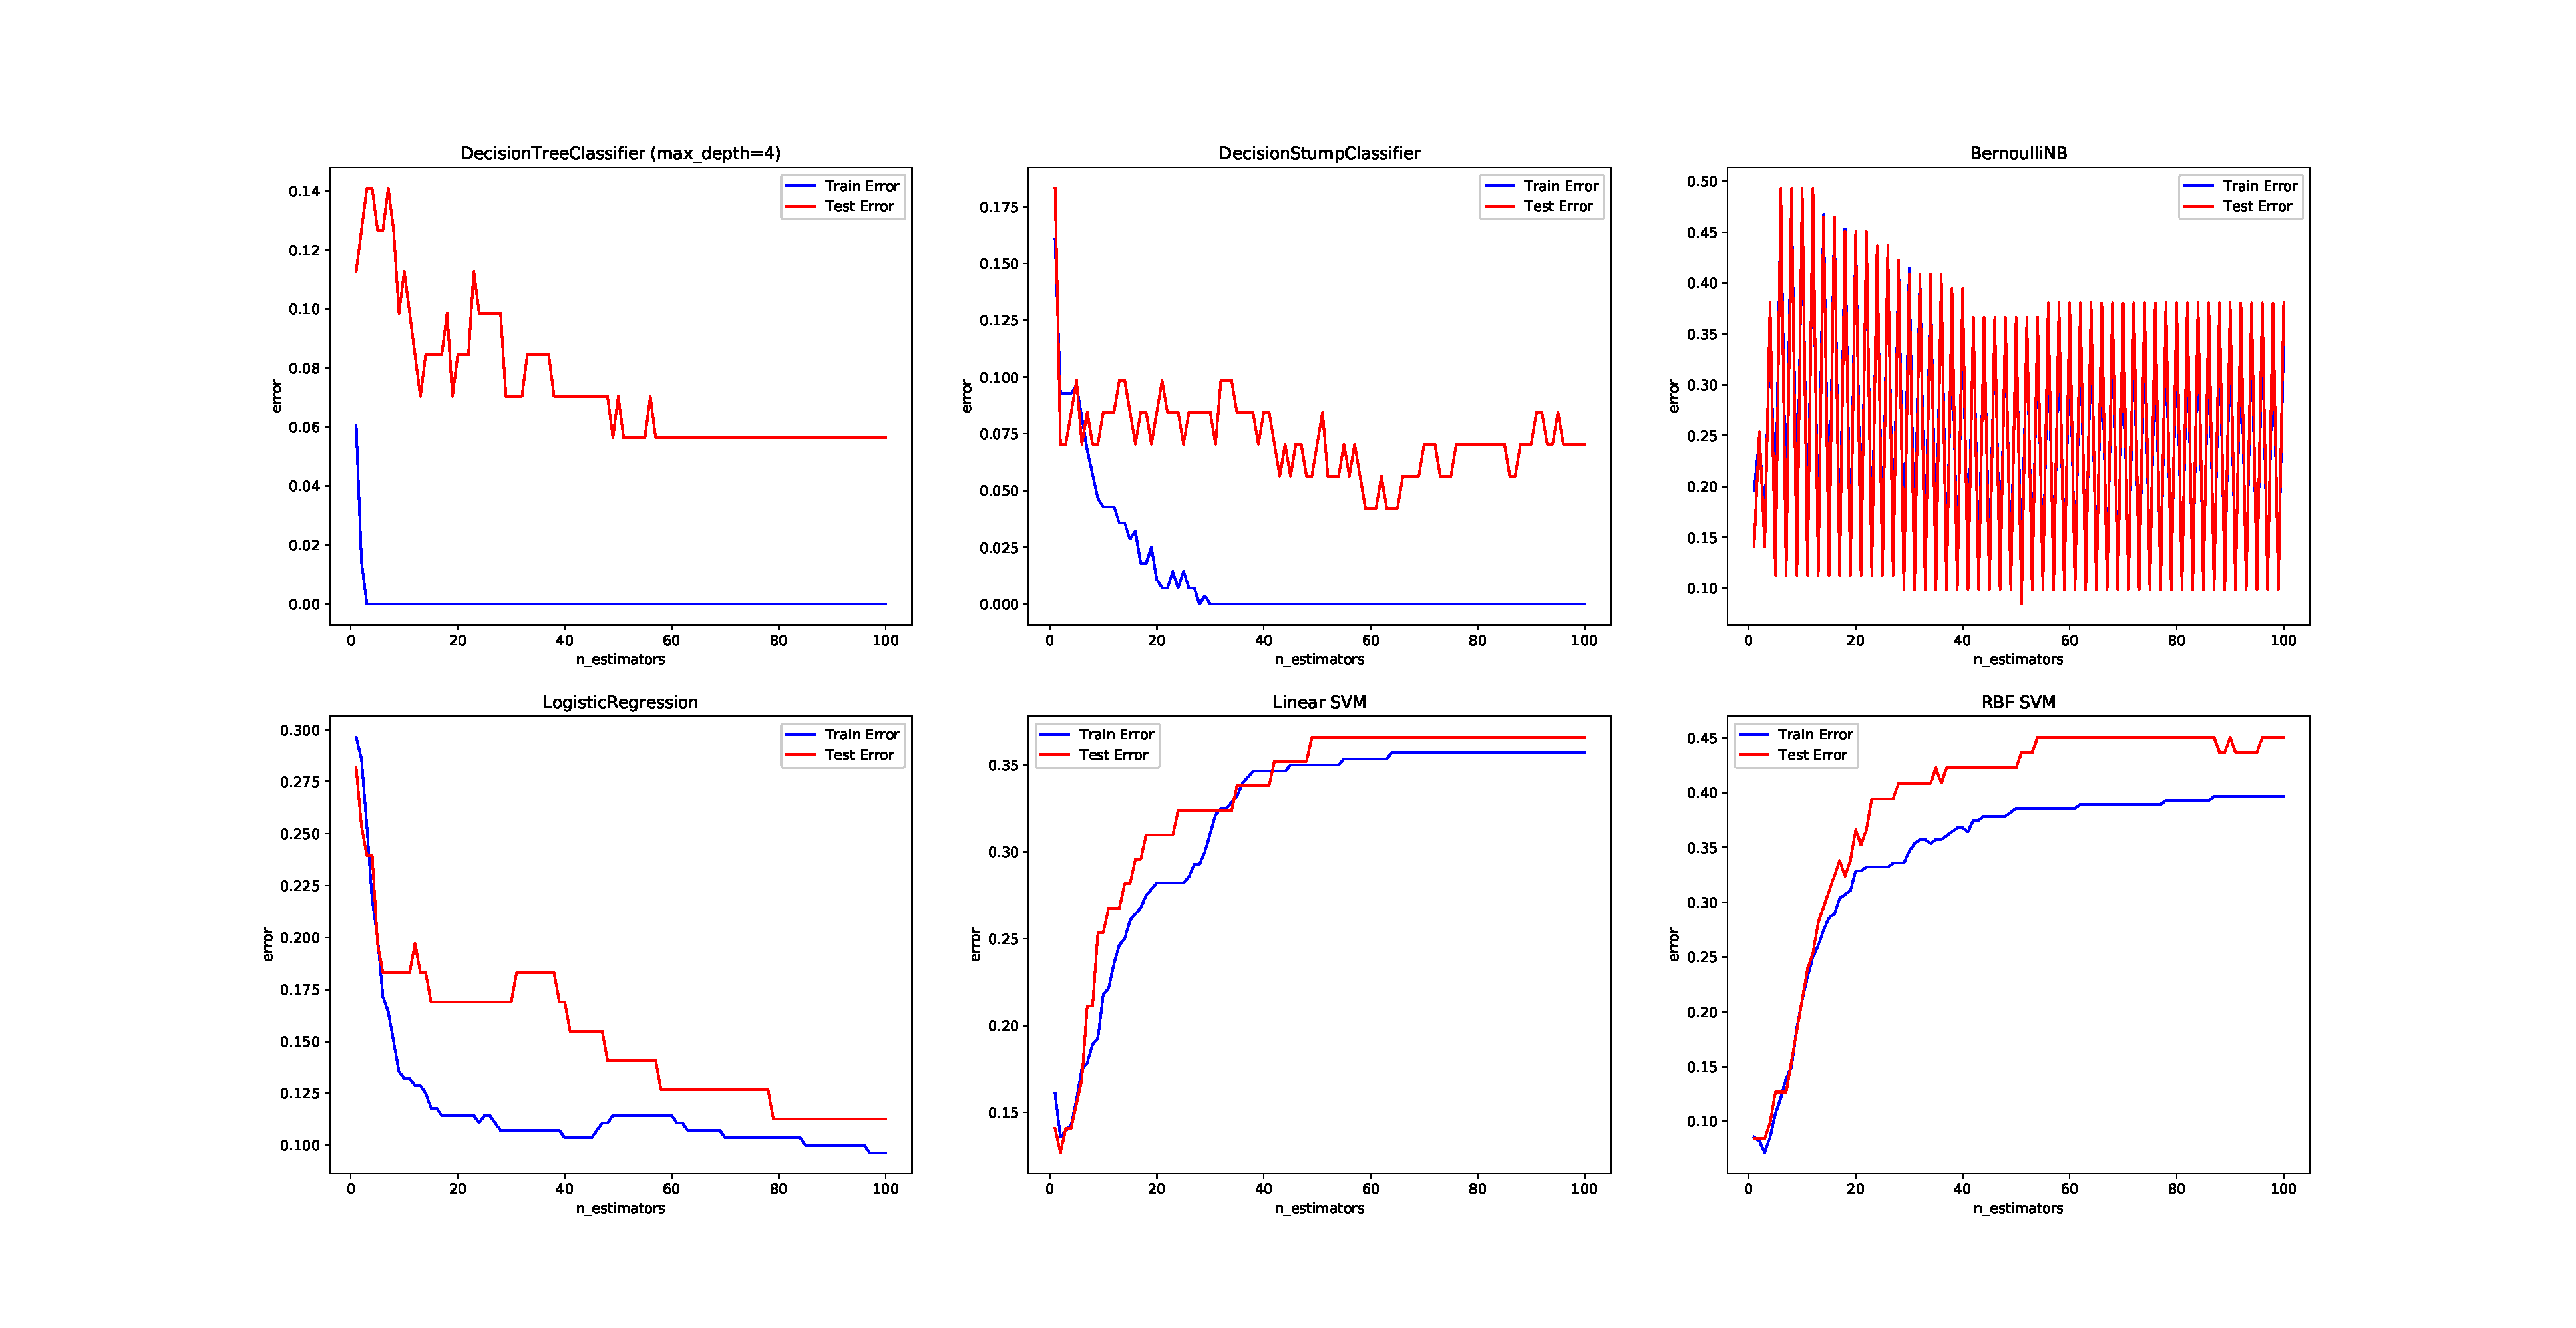
\includegraphics[width=\textwidth]{./img/adaboosterr.eps}
	\end{figure}
	
	
	\item \textbf{[3 Points]} Intuitively, is adaboost robust to overfitting? Does your results match your intuition? Why (explain in 1 - 2 sentences)?\\
	\textbf{Answer:}\\
	The adaboost is robust to overfitting, because the training and test error curves almost have the same trend with the iteration times.
	
\end{enumerate}

\subsubsection*{Submission}
For the entire programming exercise, please turn in your codes in a \textbf{single zipped folder} that contains two subfolders and each folder contains corresponding source code files for each problem.

\end{document}
